
% License:
% CC BY-NC-SA 3.0 (http://creativecommons.org/licenses/by-nc-sa/3.0/)
%
%%%%%%%%%%%%%%%%%%%%%%%%%%%%%%%%%%%%%%%%%

%----------------------------------------------------------------------------------------
%	PACKAGES AND OTHER DOCUMENT CONFIGURATIONS
%----------------------------------------------------------------------------------------

\documentclass[paper=a4, fontsize=11pt]{scrartcl} % A4 paper and 11pt font size

\usepackage[T1]{fontenc} % Use 8-bit encoding that has 256 glyphs
\usepackage{fourier} % Use the Adobe Utopia font for the document - comment this line to return to the LaTeX default
\usepackage[english]{babel} % English language/hyphenation
\usepackage{amsmath,amsfonts,amsthm} % Math packages
\usepackage{lipsum} % Used for inserting dummy 'Lorem ipsum' text into the template

\usepackage[]{algorithm2e}
\usepackage{rotating}

\usepackage{caption}
\usepackage{subcaption}
\usepackage{graphicx}
\usepackage{pgfgantt}
\usepackage{lscape}

\usepackage[utf8]{inputenc}
%\usepackage{dtklogos}
\usepackage{tikz}
\usetikzlibrary{mindmap,shadows}

\newcommand*{\info}[4][16.3]{%
  \node [ annotation, #3, scale=0.65, text width = #1em, inner sep = 2mm ] at (#2) {%
  \list{$\bullet$}{\topsep=0pt\itemsep=0pt\parsep=0pt
    \parskip=0pt\labelwidth=8pt\leftmargin=8pt
    \itemindent=0pt\labelsep=2pt}%
    #4
  \endlist
  };
}
\usepackage{latexsym}
\usepackage{amssymb,amsmath,amsthm}

\usepackage{float}

\usepackage{blindtext} %for enumarations

\usepackage[]{hyperref}  %link collor

%talbe layout to the right
%\usepackage[labelfont=bf]{caption}
%\captionsetup[table]{labelsep=space,justification=raggedright,singlelinecheck=off}
%\captionsetup[figure]{labelsep=quad}

\usepackage{sectsty} % Allows customizing section commands
%\allsectionsfont{\normalfont\scshape} % Make all sections centered, the default font and small caps

\usepackage{fancyhdr} % Custom headers and footers
\pagestyle{fancyplain} % Makes all pages in the document conform to the custom headers and footers
\fancyhead{} % No page header - if you want one, create it in the same way as the footers below
\fancyfoot[L]{} % Empty left footer
\fancyfoot[C]{} % Empty center footer
\fancyfoot[R]{\thepage} % Page numbering for right footer
\renewcommand{\headrulewidth}{0pt} % Remove header underlines
\renewcommand{\footrulewidth}{0pt} % Remove footer underlines
\setlength{\headheight}{13.6pt} % Customize the height of the header

\numberwithin{equation}{section} % Number equations within sections (i.e. 1.1, 1.2, 2.1, 2.2 instead of 1, 2, 3, 4)
\numberwithin{figure}{section} % Number figures within sections (i.e. 1.1, 1.2, 2.1, 2.2 instead of 1, 2, 3, 4)
\numberwithin{table}{section} % Number tables within sections (i.e. 1.1, 1.2, 2.1, 2.2 instead of 1, 2, 3, 4)

%\setlength\parindent{0pt} % Removes all indentation from paragraphs - comment this line for an assignment with lots of text


\setlength\parskip{4pt}

%----------------------------------------------------------------------------------------
%	TITLE SECTION
%----------------------------------------------------------------------------------------

\newcommand{\horrule}[1]{\rule{\linewidth}{#1}} % Create horizontal rule command with 1 argument of height

\newcommand{\todo}[1]{$\bigstar$ \textbf{TODO:} #1 $\bigstar$ }

\title{	
\normalfont \normalsize 
\textsc{Vienna University of Technology} \\ [25pt] % Your university, school and/or department name(s)
\horrule{0.5pt} \\[0.4cm] % Thin top horizontal rule
\huge Parallel Running Min-Max \\ % The assignment title
182.731 GPU Architectures and Computing \\
\horrule{2pt} \\[0.5cm] % Thick bottom horizontal rule
}

\author{Thomas M. Galla \& Dominik Sch\"orkhuber} % Your name

\date{\normalsize\today} % Today's date or a custom date

\begin{document}
%\nocite{*}
\maketitle % Print the title

%\newpage
\tableofcontents
\newpage

\section{Introduction and Problem Statement}

In the scope of this lab, parallel versions of a sliding window minimum/maximum filter with configurable window size inspired by a sequential algorithm developed by Lemire~\cite{lemire2006streaming} and its reference implementation\footnote{\url{https://github.com/lemire/runningmaxmin}} had to be implemented. The implementation had to be done using NVIDIA's parallel computing platform and programming model for general computing on graphical processing units (GPUs) named CUDA\footnote{\url{https://docs.nvidia.com/cuda/}}.

Hereby different versions of the algorithm (with different degrees of optimization and parallelism) have been implemented using plain CUDA on the one hand and Thrust\footnote{\url{https://docs.nvidia.com/cuda/thrust/index.html}} (NVIDIA's C++ template library for CUDA) on the other hand.
 
The source code for this project together with profiling screenshots and measurement data is publicly available at \url{https://github.com/dschoerk/GPU_Arch_SS19/}.

\section{Testing Framework and Application}
In a first step towards our implementation we implemented a framework to test and performance measure our different flavors of the sliding window minimum/maximum filter algorithm. The framework consists of several components.

First we created a common abstraction for the different algorithm implementations in form of the \texttt{streaming\_min\_max\_algorithm\_interface} interface. The interface declares a \texttt{calc} function which executes the particular algorithm. Additionally, the interface provides common functions to retrieve the computed minimum and maximum values for the sake of comparison against Lemire's reference implementation.

For each individual flavor of the algorithms (including Lemire's reference implementation) the interface was instantiated by the respective implementation and stored in an array (\texttt{algorithms\_array}). The testing framework iterates over all algorithm instances in the array for a configurable number of iterations and computes the results for all of them. Hereby the average timing for one iteration of each algorithm flavor is computed by measuring the total execution time (wall clock time of the host CPU using its high resolution clock) for all iterations and dividing this by the number of iterations. This is done as a counter measure against one-time effects during execution like cold caches etc. To properly visualize individual execution segments for a setup phase (covering the allocation of memory on the GPU device and the transfer or input data from the host CPU's memory to the memory of the GPU device), the actual processing phase (i.e., the execution of the computing kernel on the GPU device), and a tear-down phase (covering the transfer of the output data from the memory of the GPU device back to the host CPU's memory) in the NVIDIA Visual Profiler (NVVP), NVIDIA Tools Extension SDK (NVTX) Ranges are used as indicators.

As input data the framework generates uniformly distributed random samples of configurable size of floating point values in the range [-0.5,0.5]. This input data is applied to every flavor of the algorithm including Lemire's reference implementation. The output of the latter is used for a reference check to ensure the correctness of our own implementations. 

To conveniently test the algorithms, the application provides a command line interface. The sample size, window width, iterations and a verbose mode can be set with the following options:

\begin{description}
    \item[\texttt{-v (--verbose)}:] 
        Verbose mode to output additional logging. -- Only available in DEBUG builds!
    \item[\texttt{-s (--sample\_size)}:] 
        Number of elements in the input data sample.
    \item[\texttt{-w (--window\_size)}:]
        Size of the sliding window used to compute the local minima and maxima.
    \item[\texttt{-i (--iterations)}:] 
        Number of iterations to repeat the execution of every algorithm flavor. -- Very useful to actually measure consistent timings and to average out on-time effects.
\end{description}

Figure~\ref{fig:exampleoutput} illustrates an example output for a run with a sample size of $10^7$ random numbers, a sliding window size of 512 for the minimum and maximum computation, and a iteration count of 20 to generate robust results. On the bottom the average execution time for each algorithm is shown.

\begin{figure}[h]
    \centering
    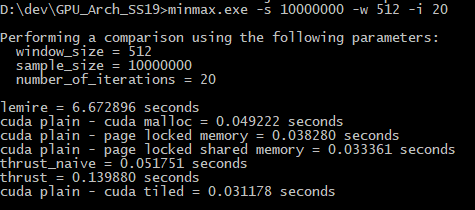
\includegraphics[width=0.8\linewidth]{Figures/exampleoutput}
    \caption{Example output of the test framework and application}
    \label{fig:exampleoutput}
\end{figure}

\section{Optimization}

When executing an algorithm on a GPU the following four typical steps are taken as illustrated in Figure~\ref{fig:steps}. As a first step memory on the GPU needs to be allocated for the input and the output data of the algorithm. In a second steps the input data is transferred from the host CPU's memory into the allocated GPU memory. In the third step, the computing kernel is executed on the GPU device using the input data in device memory and writing output data to device memory. Finally, the output data is transferred back to host memory.

\begin{figure} [h]
    \centering
    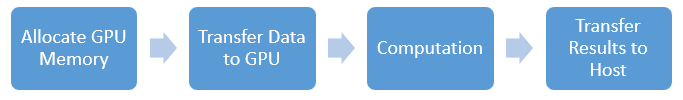
\includegraphics[width=0.8\linewidth]{Figures/steps}
    \caption{Steps to execute an algorithm on the GPU\label{fig:steps}}
\end{figure}

To create a well-performing algorithm, each step needs to be considered carefully. A naive implementation can cost several magnitudes of performance.

To maximize performance for our algorithms we pursue two orthogonal optimization strategies. First we optimize the memory transfer speed, as initial performance measurements indicated that copying the data from the host to the GPU device and back takes the largest amount of time. Secondly, we experiment with different strategies w.r.t.\ parallelization to compute the minima and maxima efficiently. 

\subsection{Memory Optimization Strategies}
\label{ch:memory optimization}

With respect to memory allocation and data transfer, a first straight-forward implementation might consider allocating memory on the GPU device using \texttt{cudaMalloc()}, transferring the input data from the host CPU to the GPU device's memory by means of \texttt{cudaMemcpy()}, executing the computation kernel on the GPU, transferring the input data from the GPU device's memory back to the host CPU by means of \texttt{cudaMemcpy()}, and finally de-allocating the memory on the GPU device by means of \texttt{cudaFree()}.

When doing this it is important to allocate and de-allocate the GPU memory en-block (allocate a large chunk of memory and divide it afterwards in smaller allocation units) in order to limit the number of \texttt{cudaMalloc()} and \texttt{cudaFree()} calls to the bare minimum to reduce the overhead that comes along with them. Similar the amount of individual \texttt{cudaMemcpy()} calls should be reduced as well if possible.

Figure~\ref{fig:memory_malloc} depicts the overhead of \texttt{cudaMalloc()} and \texttt{cudaFree()} (highlighted in yellow) as profiled on an NVIDIA Tesla K10.G2 GPU for an execution with sample size of $10^7$, a sliding window size of 500, and 3 iterations. Note that obviously the CUDA driver already performs some optimization here, since the overhead for \texttt{cudaMalloc()} is only visible in the first invocation, but not in any subsequent ones. In addition to the overhead caused by \texttt{cudaMalloc()} and \texttt{cudaFree()}, in this setup the CUDA driver has to transfer the data from pageable host memory to internally page-locked (i.e., non pageable) memory which can then serve as a source (or as the destination) of a DMA transfer between the host CPU and the GPU device causing an additional copy operation of the data in each direction.

\begin{figure}[h]
    \centering
    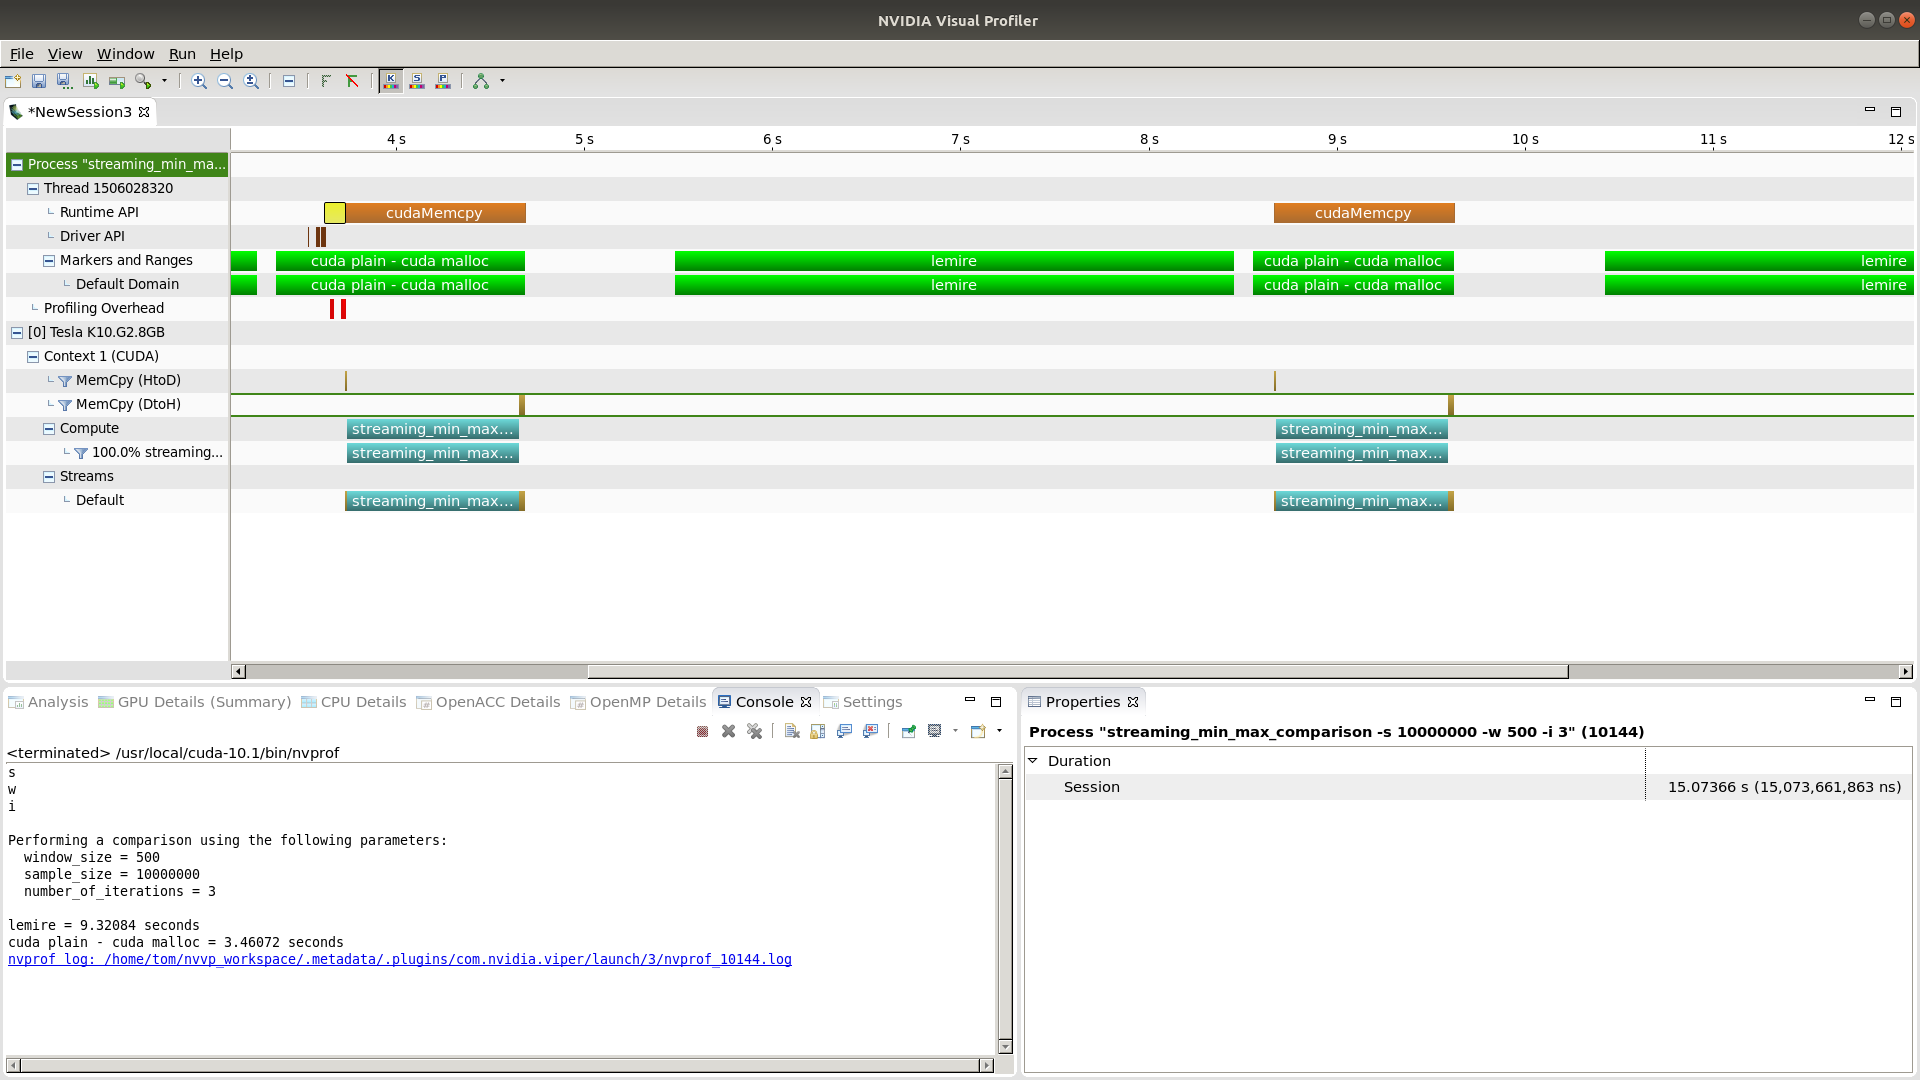
\includegraphics[width=0.8\linewidth]{Figures/memory_malloc}
    \caption{Profiling an execution with \texttt{cudaMalloc()} and \texttt{cudaFree()} \label{fig:memory_malloc}}
\end{figure}

Thus as a further improvement the logical consequence is to directly make use of \emph{page-locked host memory}. The page-locked host memory is then registered for access from the GPU device by means of \texttt{cudaHostRegister()} and \texttt{cudaHostDeregister()}. This allows the GPU to directly access the host CPU's memory and as such completely avoids the overhead of \texttt{cudaMalloc()} and \texttt{cudaFree()}. By that we remove the need for an additional copy operation in each direction.

However, since the access to the page-locked host memory then takes place in the course of the execution of the computing kernel on the GPU device, the memory access patterns heavily depend on actual structure/algorithm of the computing kernel. Hereby non-contiguous access patterns may prevent combining multiple accesses into a single bulk transfer causing a potentially severe performance penalty. Note that this is also influenced by the CUDA driver's and the GPU's capability to coalesce multiple memory accesses into a single memory transfer. 

Additionally direct access to host memory has a drawback in case a single memory location is accessed multiple times. Although this drawback can be reduced by means of caches, these usually exhibit a least-recently used (LRU) replacement strategy, which may be far from optimal for the respective memory access pattern of the computing kernel.

\begin{figure}[h]
    \centering
    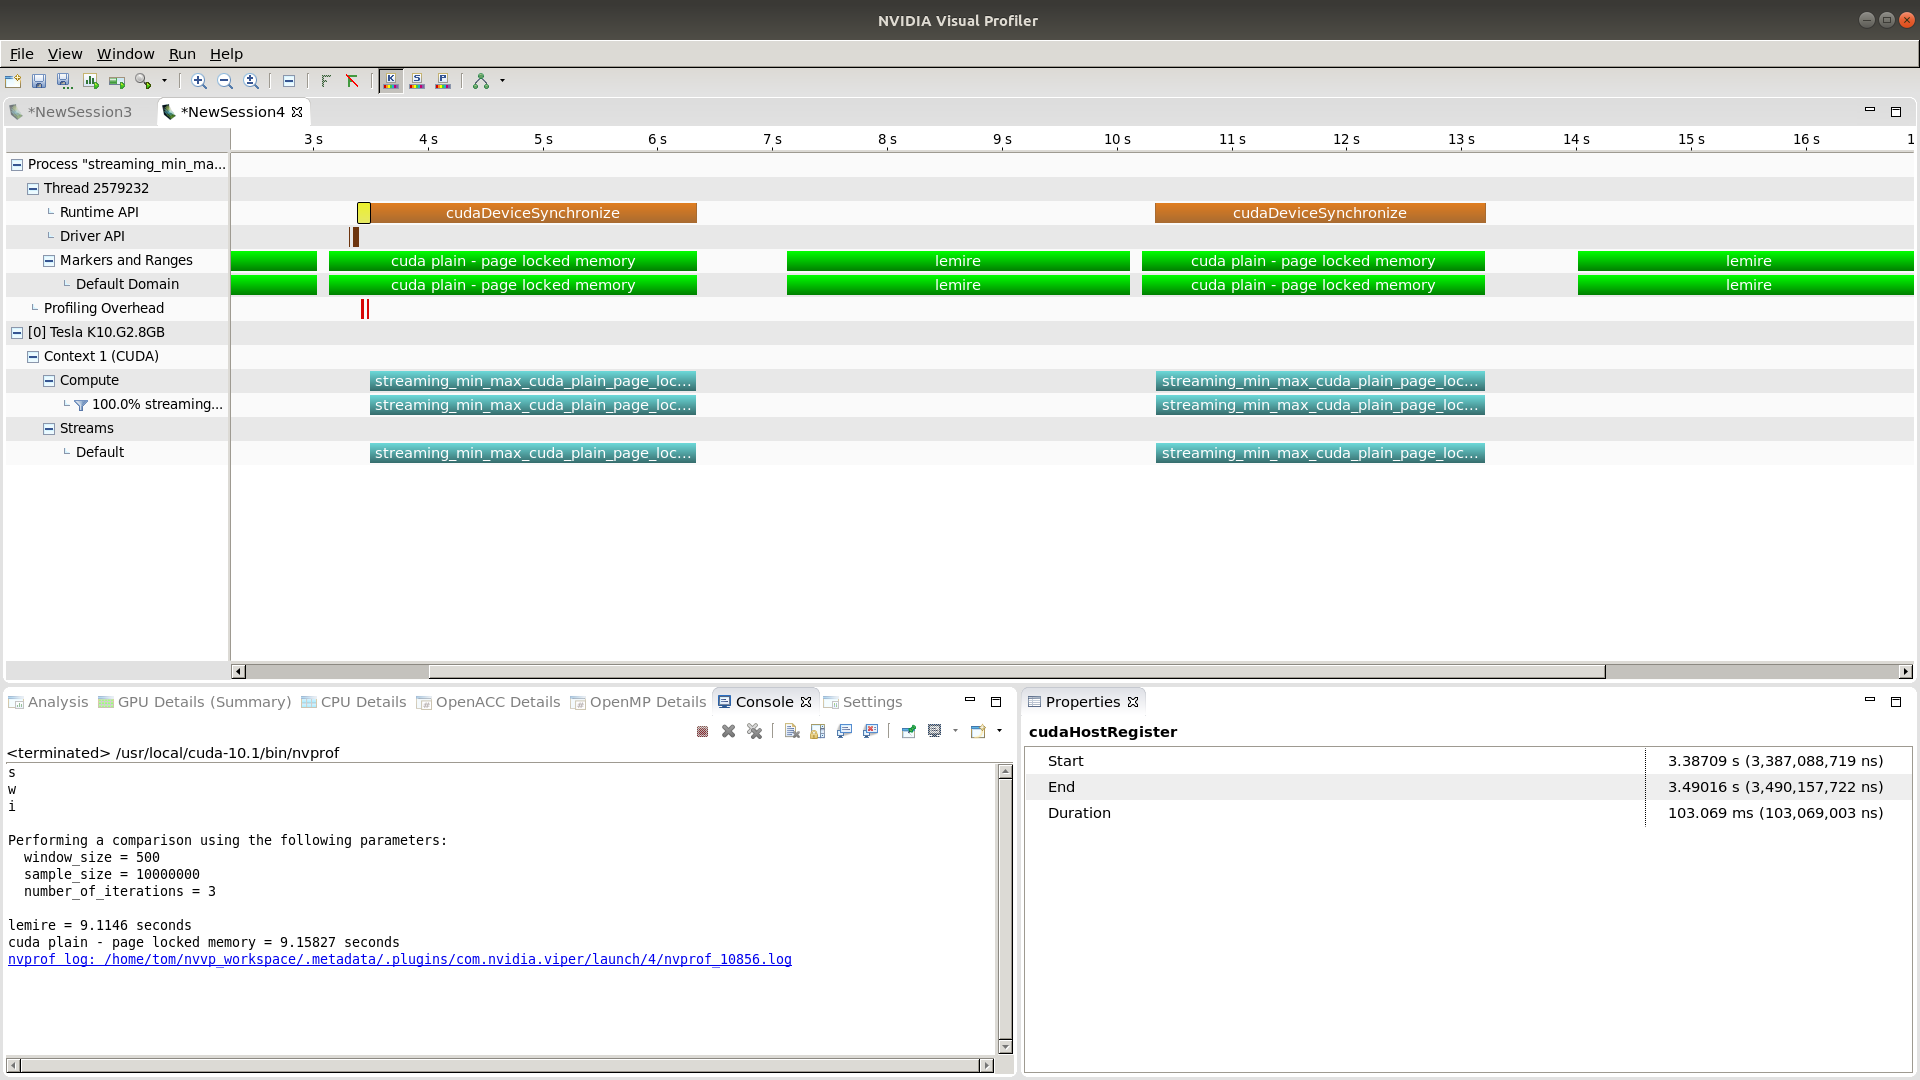
\includegraphics[width=0.8\linewidth]{Figures/memory_page_locked}
    \caption{Profiling an execution with page-locked host memory \label{fig:memory_page_locked}}
\end{figure}

Figure~\ref{fig:memory_page_locked} illustrates the a profiling run on the same NVIDIA Tesla K10.G2 GPU where the use of \texttt{cudaMalloc()} and \texttt{cudaFree()} together with \texttt{cudaMemcpy()} has been replaced by the use of page-locked host memory with \texttt{cudaHostRegister()} and \texttt{cudaHostDeregister()}. -- For this profiling run the same arguments, namely a sample size of $10^7$, a sliding window size of 500, and 3 iterations have been used. Similar to the previous profiling run, the overhead caused (this time by \texttt{cudaHostRegister()}) is highlighted in yellow. Looking at the execution times as well as on the profiling chart it becomes obvious that at least on this NVIDIA Tesla K10.G2 GPU, this ``optimization'' in fact is a severe deterioration w.r.t.\ performance.

To overcome the performance penalty when directly accessing page-locked host memory (even with caching in place), the use of \emph{shared memory}, which is as performant as the GPU's streaming multiprocessor's L1 cache and shared amongst the different threads of a thread block as a kind of \emph{program-controlled cache} is possible. Hereby the transfer between the page-locked host memory and the GPU's shared memory is performed under the control of the computing kernel and may thus be aligned with the concrete memory access pattern of the computing kernel.

Figure~\ref{fig:memory_shared} illustrates a profiling run on the same hardware as the previous two where the use of page-locked host memory with \texttt{cudaHostRegister()} and \texttt{cudaHostDeregister()} has been complemented with the use of shared memory as program-controlled cache.

\begin{figure}[h]
    \centering
    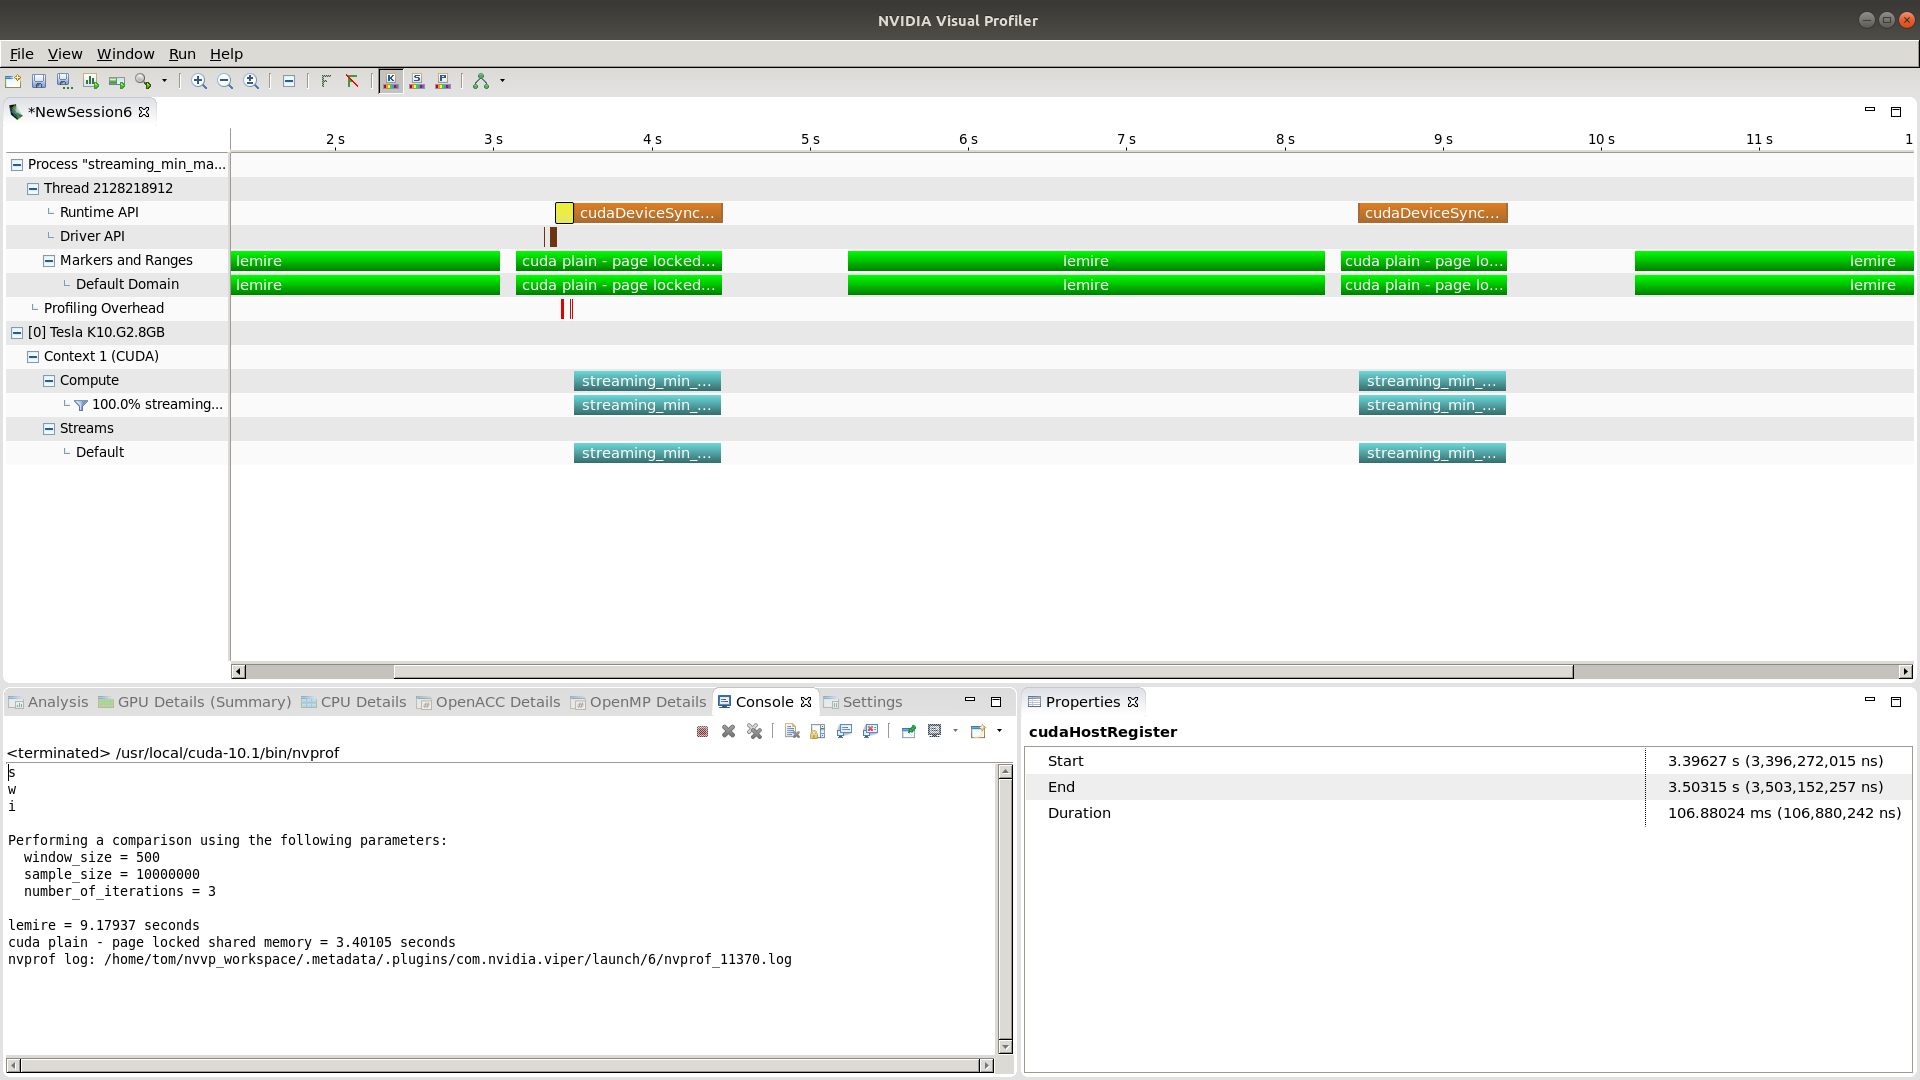
\includegraphics[width=0.8\linewidth]{Figures/memory_shared}
    \caption{Profiling an execution with page-locked host memory using shared memory as program-controlled cache\label{fig:memory_shared}}
\end{figure}

\subsection{Parallelization Strategies}
\label{ch:parallelization}
We are pursuing two different parallelization strategies to find the minimum and maximum values within a window. In our first strategy we compute each sliding window by one thread. The thread iterates over all values in the current window and computes the result step by step. This approach is used by the CUDA Malloc, CUDA Page-Locked, CUDA Page-Locked Shared, and Thrust Naive implementations and is illustrated in Algorithm~\ref{alg:linearscan}.

\begin{algorithm}[h]
    \KwData{w = window size, s = data size}
    \For{each thread k in parallel}{
        minimum = input[k] \\
        maximum = input[k] \\
        \For{each position $i$ in a window of length $w$}{
            minimum = min(minimum, input[k + i]) \\
            maximum = max(maximum, input[k + i]) \\
        } 
        $\mathrm{minima}_{\mathrm{out}}$[k] = minimum \\
        $\mathrm{maxima}_{\mathrm{out}}$[k] = maximum
    }
    \caption{Linear scan}
    \label{alg:linearscan}
\end{algorithm}

However, we found that the reduction step of our min/max algorithm shares some properties with the prefix sum algorithm. A naive scheme to compute the prefix sum is shown in  Figure~\ref{fig:prefixsum}.

\begin{figure}[h]
    \centering
    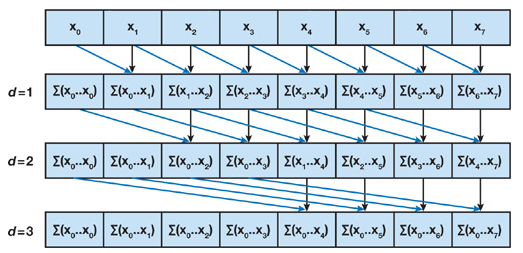
\includegraphics[width=0.6\linewidth]{Figures/prefix}
    \caption{Naive computation of prefix sum~\cite{Nguyen:2007:GG:1407436}}
    \label{fig:prefixsum}
\end{figure}

We recognize that in such a binary reduction scheme the number of summed values doubles in each step, i.e., the number of summed values per node in a level $d$ is $2^d$. Following this observation we can replace the plus operator with the min/max functions and therefore compute the min/max values for all windows of size $2^d$. To now compute windows of arbitrary length $w$ we can combine the min/max results of the next smaller power of 2 sized window length, and fall back to our linear scheme presented previously to perform the combination. This approach is taken in the Thrust and CUDA Tiled implementations. A better depiction of this scheme is shown in Figure~\ref{fig:prefixsum2}.

\begin{figure}[h]
    \centering
    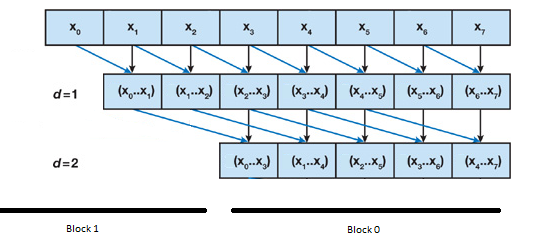
\includegraphics[width=0.8\linewidth]{Figures/prefix2}
    \caption{Naive prefix sum adapted to the min/max problem. The example shows a block size of 8. For $d=2$ four input numbers are required for each output cell. The three left most cells cannot output a number, but must be overlapped with the next block.}
    \label{fig:prefixsum2}
\end{figure}

Here we can intuitively see that not all threads can contribute a final output value, instead in each level the number of threads contributing to the output directly is reduced by $2^d-1$. The output size that can be computed by a block of length $n$ is $n - w + 1$. Therefore the blocks in the computation grid must be overlapped by $w - 1$ units. This remains true for arbitrary window lengths. The computation and indexing scheme is shown in Algorithm~\ref{alg:loglinearscan}. For the sake of simplicity we have left out tiling over multiple blocks in this pseudo code.

\begin{algorithm}[h]
    \KwData{w = window size, s = data size}
    \For{each thread k in parallel}{
        \For{d = 0; d < $\lfloor log_2(w) \rfloor$; d++}{
            \If{$k + 2^d < s$}{
                minima[k] = min(minima[k], minima[k + $2^d$] \\
                maxima[k] = min(maxima[k], maxima[k + $2^d$] \\
            }
        }
        
        \If{k < s - w + 1} {
            minimum = minima[k] \\
            maximum = maxima[k] \\
            \For{i=0; i < w - $\lfloor log_2(w) \rfloor$; i++}{
                minimum = min(minimum, input[k + i + 1]) \\
                maximum = max(maximum, input[k + i + 1]) \\
            } 
            $\mathrm{minima}_{\mathrm{out}}$[k] = minimum \\
            $\mathrm{maxima}_{\mathrm{out}}$[k] = maximum
        }
    }
    \caption{Log linear scan}
    \label{alg:loglinearscan}
\end{algorithm}

\section{Implementations}
In this section we briefly explain the differences and implementation details for each of the algorithms. We can broadly categorize the algorithm implementations by the usage of Thrust and plain CUDA. 

\subsection{Thrust Naive}
\label{sec:thrust_naive}
In this implementation making use of thrust, we have first attempted to utilize the provided reduction schemes in Thrust as much as possible. A parallel reduction is provided by the Thrust library with \texttt{thrust::minmax\_element}. While this function computes the min/max elements over a given range, it requires us to rerun the function for each shifted window and thus result in a prohibitive amount of kernel calls\footnote{\url{https://github.com/dschoerk/GPU_Arch_SS19/blob/master/streaming\_min\_max\_thrust\_naive\_cuda.cu\#L97-L107}}.  We have therefore shifted strategies and (ab)use \texttt{thrust::foreach} on a counting iterator spanning $s - w + 1$ elements and implement Algorithm~\ref{alg:linearscan} in a functor to run by the foreach thrust call. 

\subsection{Thrust}
In the second thrust based implementation we follow the same strategy which is based on \texttt{thrust::foreach} and a counting iterator for parallelization. However, in this version we implement the (in theory) more efficient computation scheme of Algorithm~\ref{alg:loglinearscan}. To achieve grid wide synchronization for each $2^d$ span, we need to run them as separate kernels. An attempt to synchronize via cooperative groups\footnote{\url{https://docs.nvidia.com/cuda/cuda-c-programming-guide/index.html\#cooperative-groups}} failed for various reasons and is explained below. The fallback to running separate kernels introduces again a big overhead w.r.t.\ computation time. While the code for both thrust implementations is very readable, their performance is not on par with the plain CUDA implementations.

\subsubsection{Synchronization with Cooperative Groups}
In an experiment we tried to utilize the cooperative group feature to achieve grid wide synchronization. Using cooperative groups failed for various reasons. First research showed that a GPU with at least compute capability 3.5 is required to make use of cooperative groups. At least the RTX 2070 would suffice that. However, further research revealed additional constraints. Either a Linux system without MPS\footnote{\url{https://docs.nvidia.com/deploy/mps/index.html}}, or a Windows system with the GPU in TCC (instead of WDDM) mode\footnote{\url{https://docs.nvidia.com/gameworks/content/developertools/desktop/nsight/tesla_compute_cluster.htm}} must be used. Since the RTX 2070 is the only video card in the used desktop system it was not possible to run it in TCC (headless) mode. Furthermore it is required to launch the kernels with \texttt{cudaLaunchCooperativeKernel} which might not be the case for Thrust. Nevertheless it was an interesting experiment and may be useful for other implementations in the future. Especially as a replacement to global block synchronization hacks as described in the lectures. 

\subsection{CUDA Malloc}
\label{sec:cuda_malloc}
This implementation is a plain CUDA implementation (not using Thrust or CUDA streams) which only makes use of \texttt{cudaMalloc()} and \texttt{cudaFree()} and explicit data transfer between the host CPU and the GPU device via \texttt{cudaMemcpy()} (i.e., it does not use page-locked and/or shared memory).

From a parallelization strategy perspective, this implementation pursues the first presented strategy, namely one thread per min/max output and thus renders this implementation the plain CUDA counter part to the Thrust Naive implementation presented in Section~\ref{sec:thrust_naive}.

\subsection{CUDA Page-Locked}
\label{sec:cuda_page_locked}
In contrast to the CUDA Malloc implementation described in Section~\ref{sec:cuda_malloc}, this implementation makes use of page-locked host memory (albeit without using shared device memory as a cache). Thus the memory containing the input and output vectors of the algorithms are registered for GPU device access (and thereby page-locked) with \texttt{cudaHostRegister()} (and de-registered via \texttt{cudaHostDeregister()} after use).

From the parallelization strategy perspective, this implementation is identical to the CUDA Malloc implementation described in Section~\ref{sec:cuda_malloc}.

\subsection{CUDA Page-Locked Shared}
In addition to the CUDA Page-Locked implementation described in Section~\ref{sec:cuda_page_locked}, this implementation uses of the GPU's shared memory as a program-controlled cache. Hereby for every thread block a chunk of shared memory is statically allocated. The execution of the computing kernel is divided into two phases. In the first phase the shared memory of every thread block is filled element-wise (one element per thread) in parallel with the input data which is afterwards worked on by this thread block. In the second phase the actual processing of the input data (i.e., the computation of the sliding window minimum/maximum algorithm) takes place and purely acts on the data cached in the shared memory.

From the parallelization strategy perspective, this implementation is as well identical to the CUDA Malloc implementation described in Section~\ref{sec:cuda_malloc}.

\subsection{CUDA Tiled}
In this implementation we have combined the effects of the superior page-locked memory with shared GPU memory as a program-controlled cache and the advanced computation scheme in Algorithm~\ref{alg:loglinearscan}. To enable sample vectors of arbitrary length and avoid the cost of grid wide synchronization, we implement a tiling scheme.

The tiling scheme operates on a per block level such that synchronization is only required within a block and can be achieved with \texttt{\_\_syncthreads}. The tiling scheme is further illustrated in Figure~\ref{fig:tiled}. The number of output values is bounded by the block size $b$ as described in Chapter~\ref{ch:parallelization} to $b - w + 1$. We therefore overlap blocks accordingly to receive $s - w + 1$ output values in total. This requires re-computation of some values already present in a previous block, but is overall more efficient than a costly grid wide synchronization step.

\begin{figure} [h]
    \centering
    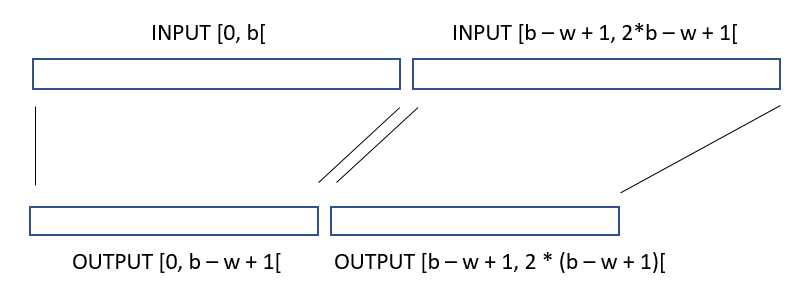
\includegraphics[width=0.8\linewidth]{Figures/tiling}
    \caption{Tiling schema to avoid grid wide synchronization. Some computed values in the overlapping regions are lost and need to be re-computed by the next block.}
    \label{fig:tiled}
\end{figure}

\section{Results and Comparison}

In this chapter we are describing how we have tested and benchmarked our implementations. We have tested the different flavors of the algorithm on two different test systems. The first system is the department's test system with a Tesla K10.G2 GPU, and the second system is a personal computer with an NVIDIA RTX 2070 GPU.

We evaluate the implemented approaches by providing benchmarks with different sample and window sizes and discuss the differences between the chosen strategies as well as differences regarding the two GPU's.

\subsection{NVIDIA RTX 2070}

The overview in Figure~\ref{fig:group_picture_rtx2070} shows the output of NVIDIA's visual profiler (NVVP) executed on the RTX 2070 test system. The green bars are marking the full computation time for each algorithm. This includes the allocation of host memory (unmarked).

\begin{sidewaysfigure}
    \centering
    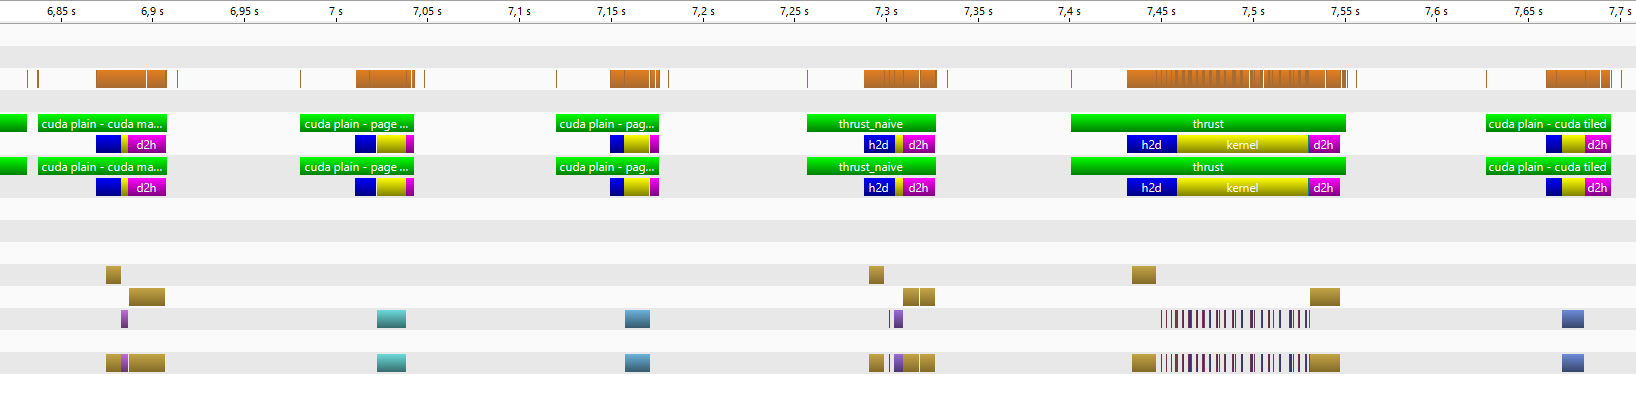
\includegraphics[width=1.0\linewidth]{Figures/group_picture_rtx2070}
    \caption{Overview of algorithms for a profiling run with a sample size of $10^7$ and a sliding window size of 256 on the NVIDIA RTX 2070. NVTX ranges are marking the phases of each algorithm. Preparation time in blue. Kernel execution in yellow. Copying results to host in pink. Shown from left to right are: CUDA Malloc, CUDA Page-Locked, CUDA Page-Locked Shared, Thrust Naive, Thrust, and CUDA Tiled}
    \label{fig:group_picture_rtx2070}
\end{sidewaysfigure}

The allocation and transfer of/to device memory (blue), the kernel execution (yellow) and transferring the results from device to host memory (pink).

Without going into the detailed numbers, we can see that the time taken for memory allocations and transfer dominates the timescale. Typically the kernel execution only takes a quarter of the overall processing time (except for the thrust implementation). 

What we can also see in this overview is that multiple kernel calls are computation wise extremely expensive, but sometimes needed to achieve a grid wide synchronization as required in the Thrust implementation (Figure~\ref{fig:group_picture_rtx2070} \#5). Multiple kernels thus should be avoided at all cost, and be replaced by tiling schemes which limit the requirements for synchronization to sub groups of blocks or even warps as used in the CUDA Tiled approach (Figure~\ref{fig:group_picture_rtx2070} \#6). 

Figure~\ref{fig:rtx2070_ms_vs_samples} shows the benchmark results for the NVIDIA RTX 2070 GPU with window sizes of 100, 500, 800 and 1000 elements. We left out Lemire's approach for a better scaling of the graph. The clearly worst performing algorithm of ours was the Thrust implementation. Since global synchronization via multiple sequential kernel starts was required, the performance of this approach took a big hit. The other five approaches are performing very similarly. For smaller window sizes (100, 500) the CUDA Tiled approach performs fastest by a small margin. For larger windows (800, 1000) the naive iteration scheme performs better, and among these CUDA Page-Locked Shared is always the fastest one.

\begin{figure}[p]
    \centering
    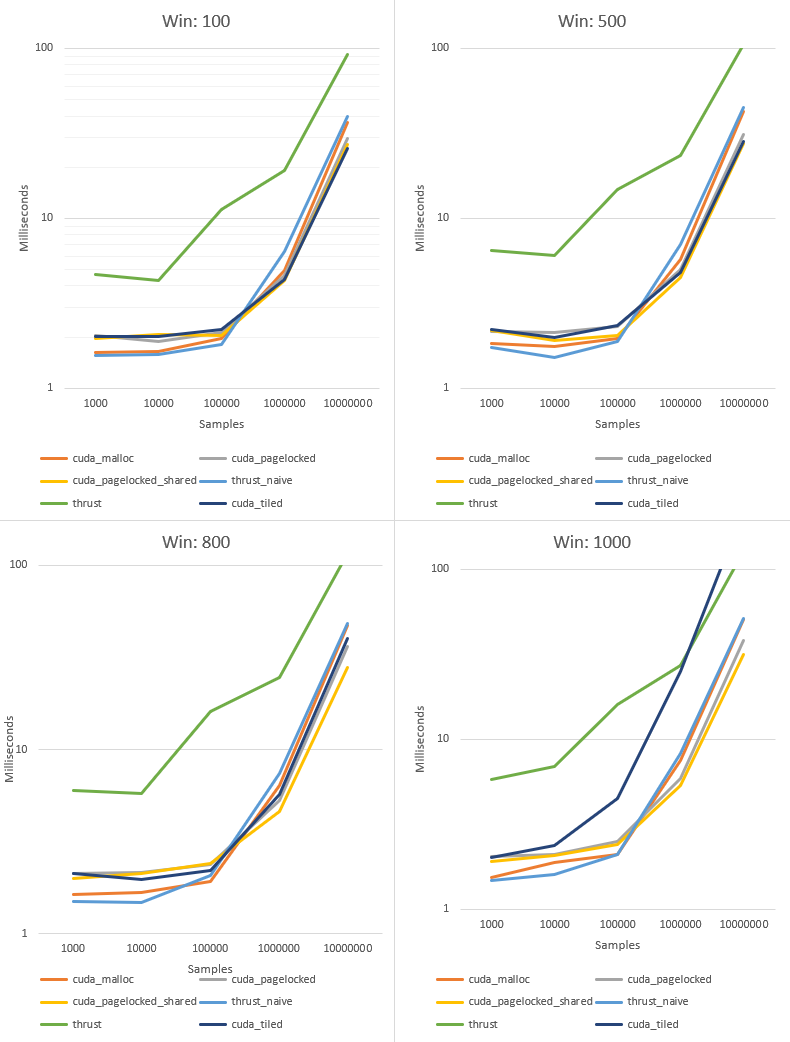
\includegraphics[width=1.0\linewidth]{Figures/rtx2070_ms_vs_samples.png}
    \caption{Results for all six implementations at different window and sample sizes. We omitted Lemire as it is much slower than competitors. Duration is shown on a logarithmic scale. The \texttt{cuda\_tiled} approach appears to be very efficient for large sample sizes and small window sizes, the naive linear scan used by \texttt{cuda\_pagelocked\_shared} dominates at large window sizes.}
    \label{fig:rtx2070_ms_vs_samples}
\end{figure}

\subsection{NVIDIA Tesla K10.G2}

The overview in Figure~\ref{fig:group_picture_tesla_k10g2} shows the output of the NVIDIA's visual profiler (NVVP) executed on the Tesla K10.G2 test system. Similar to the overview for the RTX 2070 test system the green bars are marking the full computation time for each algorithm. Again this includes the allocation of host memory (unmarked). The allocation and transfer of/to device memory (blue), the kernel execution (yellow) and transferring the results from device to host memory (pink).

\begin{sidewaysfigure}
    \centering
    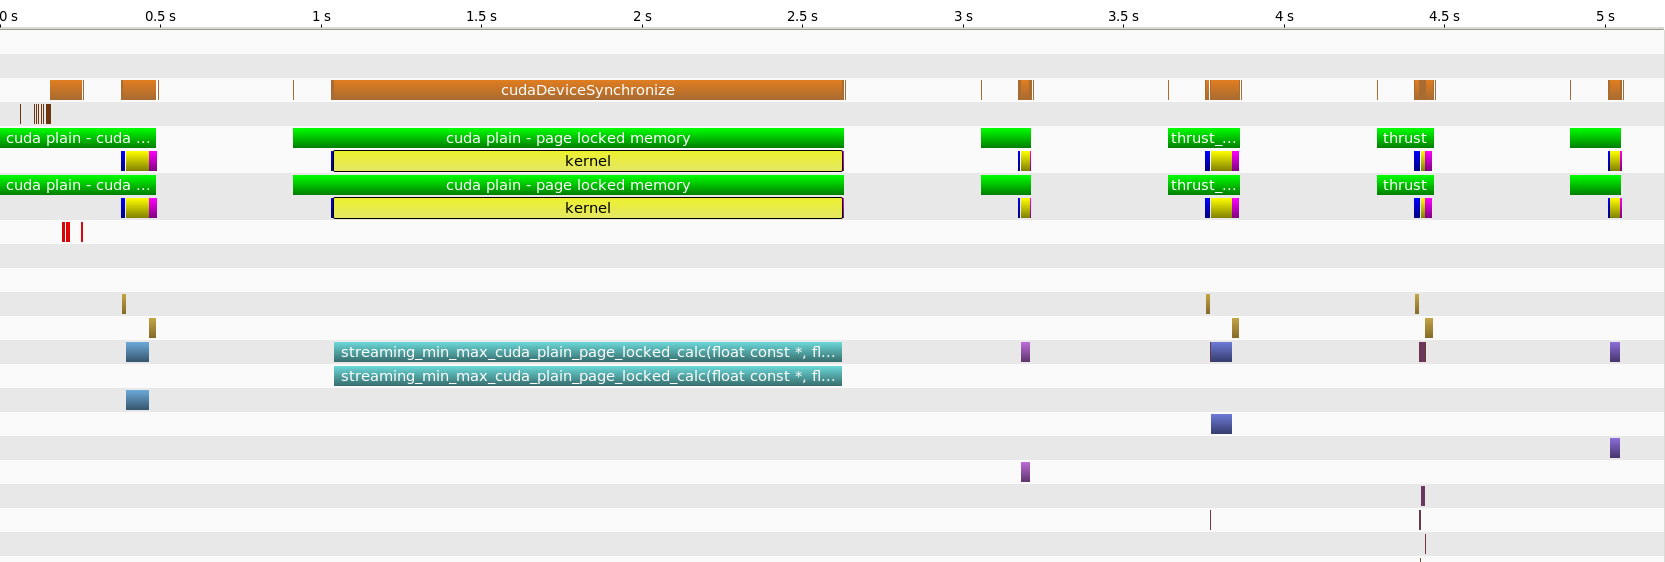
\includegraphics[width=1.0\linewidth]{Figures/group_picture_tesla_k10g2}
    \caption{Overview of algorithms for a profiling run with a sample size of $10^7$and a sliding window size of 256 on the NVIDIA Tesla K10.G2. NVTX ranges are marking the phases of each algorithm. Preparation time in blue. Kernel execution in yellow. Copying results to host in pink. Shown from left to right are: CUDA Malloc, CUDA Page-Locked, CUDA Page-Locked Shared, Thrust Naive, Thrust, and CUDA Tiled}
    \label{fig:group_picture_tesla_k10g2}
\end{sidewaysfigure}

An obvious overall difference is that all measured times on the 
Tesla K10.G2 test system are substantially (factor 2-3) longer than those measured on the RTX 2070 test system, which is not surprising considering the hardware specifications of both. Thus we'll now focus on relative differences between the two systems.

In contrast to the results from RTX 2070 test system the time required for memory allocation and memory transfer is not at all that dominating. However, the direct access to page-locked memory on the host CPU (which manifests itself in the kernel execution time of the CUDA Page-Locked implementation) dominates the timing by at least an order of magnitude. A wild guess (which is not confirmed) is that the Tesla K10.G2 test system is inferior when it comes to coalescing multiple memory accesses into a single bulk transfer. Another interesting difference is that the Thrust implementation is en-par with both plain CUDA implementations using shared memory for caching (which suggests that on the Tesla K10.G2 test system the Thrust library performs a similar caching under the hood). A final difference is that the Thrust implementation outperforms Thrust Naive implementation  on the Tesla K10.G2 test system whereas on the RTX 2070 test system it's exactly the other way round.

\begin{figure}[p]
    \centering
    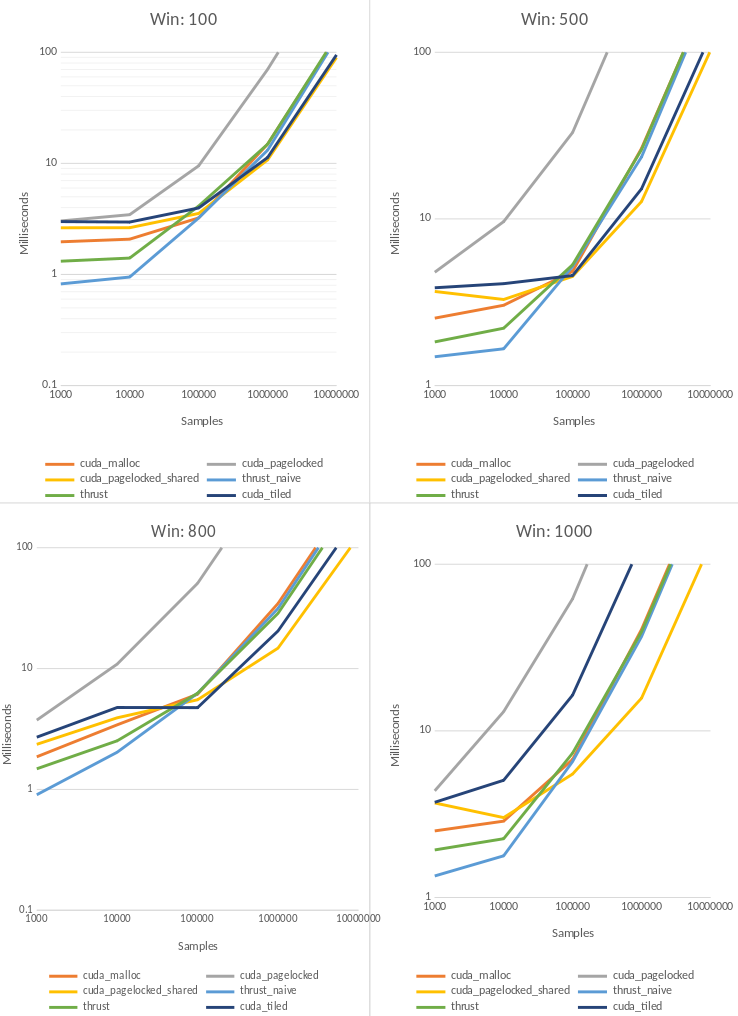
\includegraphics[width=1.0\linewidth]{Figures/tesla_k10g2_ms_vs_samples.png}
    \caption{Results for all six implementations at different window and sample sizes. Again we omitted Lemire as it is considerably slower than competitors with large sample sets. Duration is shown on a logarithmic scale. The \texttt{cuda\_pagelocked} approach (using the naive linear scan) is non-performing for all sample and small window sizes. The \texttt{cuda\_pagelocked\_shared} (which uses the naive linear scan as well) dominates at large window sizes.}
    \label{fig:tesla_k10g2_ms_vs_samples}
\end{figure}

Figure~\ref{fig:tesla_k10g2_ms_vs_samples} shows the benchmark results for the NVIDIA Tesla K10.G2 GPU with window sizes of 100, 500, 800 and 1000 elements. Again we left out Lemire's approach for a better scaling of the graph. The clearly worst performing algorithm on this test system was the CUDA Page-Locked implementation (without using shared memory as a cache) for all sample and sliding windows sizes. The hypothesized cause of this is the lack of capability to coalesce multiple memory accesses into a single bulk transfer. The CUDA tiled implementation showed the second worst performance for small sample sizes, but gains on larger samples sizes as long as the window size is below a threshold of approx.\ 900. With larger sample sizes the CUDA Page-Locked Shared implementation clearly shows the best performance.

\section{Summary \& Conclusion}

In the scope of this lab, we implemented several different flavors of a parallel version of a sliding window minimum/maximum filter with configurable window size using NVIDIA’s parallel computing platform and programming  model  for general computing on graphical processing units (GPUs) named  CUDA. These various implementation exploited different strategies w.r.t.\ performance optimizations. We conducted comprehensive measurements with different sample sizes and various sizes of the sliding window on two different hardware platforms.

The comparison of the measurement results were not fully conclusive across these two hardware platforms meaning that optimization strategies that are beneficial for one hardware platform were counter productive for the other. One common outcome on both hardware platforms however was that a rather naive parallelized linear scan together with the use of page-locked host memory combined with shared GPU memory as a program controlled cache performed superior for larger sample sizes and all window sizes on both hardware platforms.

The substantial differences in the measurement results on the two hardware platforms w.r.t.\ the merit of certain optimization strategies clearly suggest that pursuing a hybrid approach, i.e., providing various different kernel implementations within a single executable and selecting the appropriate one during run-time based on the concrete workload and the concrete hardware platform, is feasible and beneficial when striving for optimal performance on a broad range of different hardware platforms and when dealing with various different workloads.



% \input{Introduction.tex}
% \input{StateoftheArt.tex}
% \input{annotation_definition.tex}
% \input{mindmap.tex}
% \input{annotation_experiment.tex}
% \input{milestones.tex}
% \input{ideas.tex}

%bibliography
\bibliographystyle{alpha}
\bibliography{refs.bib}

\end{document}